\documentclass{article}

\usepackage[english]{babel}
\usepackage[margin=3cm]{geometry}
\usepackage{graphicx}
\usepackage{float}
\usepackage{caption}
\usepackage{hyperref}
\usepackage{amsmath}
\usepackage{wrapfig}
\usepackage[parfill]{parskip}

% fonts
\usepackage[T1]{fontenc}
\usepackage{helvet}
\renewcommand{\familydefault}{\sfdefault}

\graphicspath{{img/}}

% theorem environment
\usepackage{amssymb}

\newtheorem{theorem}{Definition}[section]

\usepackage{enumitem}

\newenvironment{thmenum}
 {\begin{enumerate}[label=\upshape\bfseries(\roman*)]}
 {\end{enumerate}}


% code
\usepackage{minted}
\setminted{frame=single,framesep=3pt,linenos}
\usepackage{upquote}
\usepackage{color}

\begin{document}

\begin{titlepage}
    \author{Tuur Vanhoutte}
    \title{Deep Learning}
\end{titlepage}

\pagenumbering{gobble}
\maketitle
\newpage
\tableofcontents
\newpage

\pagenumbering{arabic}

\section{Introduction to neural networks}

\begin{figure}[H]
    \centering
    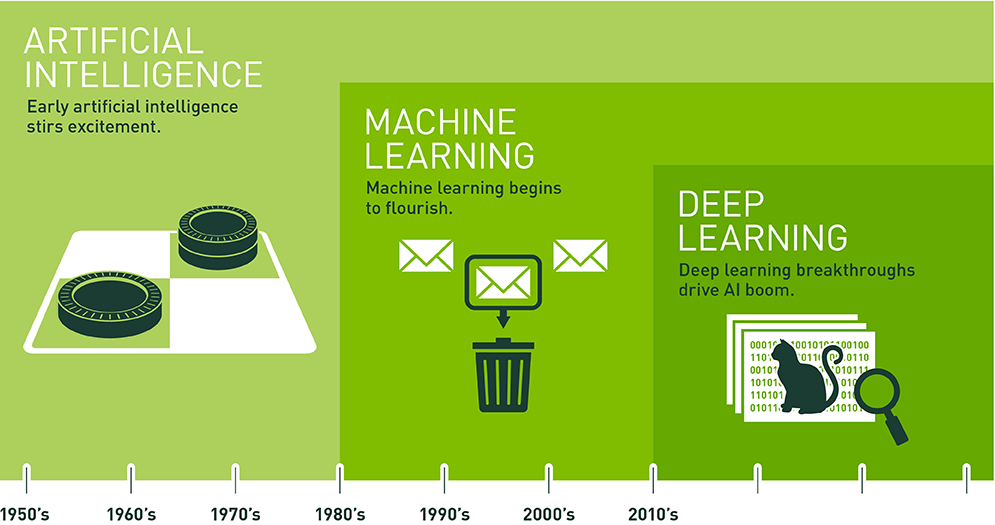
\includegraphics[width=0.6\textwidth]{ai-timeline.png}
    \caption{Timeline of AI}
\end{figure}

\subsection{Why deep learning?}

\begin{figure}[H]
    \centering
    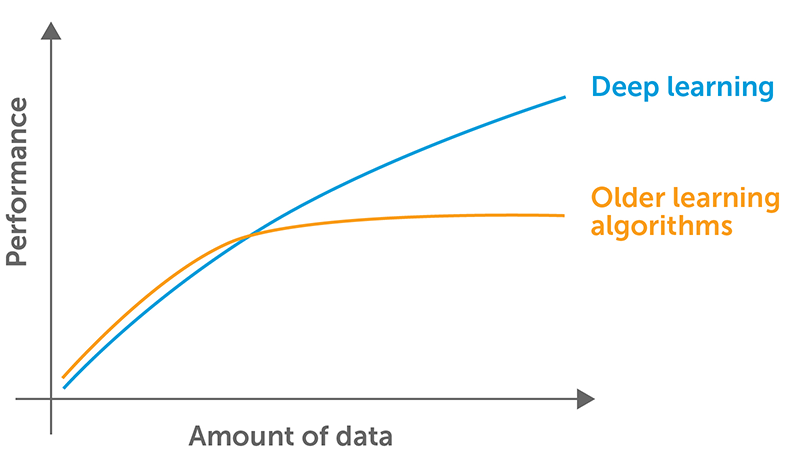
\includegraphics[width=0.5\textwidth]{deep-learning-performance-vs-data.png}
    \caption{Performance vs amount of data}
\end{figure}

\begin{itemize}
    \item The more data you have, the better the model
    \item In reality, older algorithms will plateau after a certain point
    \item With deep learning, this is much less of a problem
    \item However, neural networks are much more sensitive to overfitting: they can memorize the entire dataset
    \item For smaller datasets, it's often better to use traditional learning algorithms
\end{itemize}

\begin{figure}[H]
    \centering
    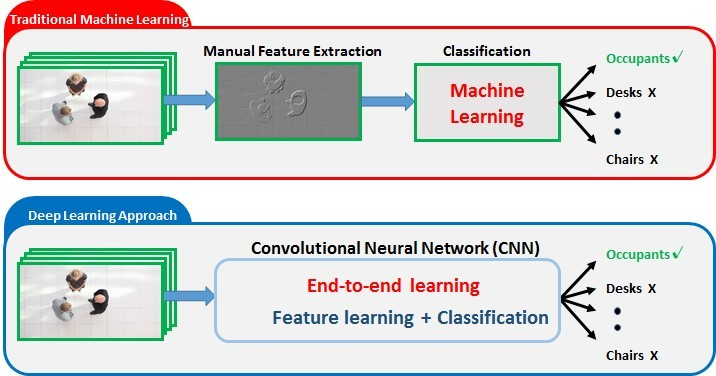
\includegraphics[width=0.7\textwidth]{deep-learning-approach.png}
    \caption{The difference in approach between traditional ML and Deep Learning}
\end{figure}

\begin{itemize}
    \item With traditional ML, you first need to extract the features manually 
    \item In the past, you had to manually mark facial features for facial recognition algorithms (eyes, mouth, ears, \dots)
    \item Deep learning is great for problems with non-structured data
    \begin{itemize}
        \item Structured data = rows of data (like an Excel-sheet)
        \item Non-structured = images, video, audio
    \end{itemize}
\end{itemize}

\begin{theorem}
    End-to-end learning is a deep learning technique where we run all raw data through a neural network.
    The neural network will do its own feature extraction (feature learning), and then a classifier will output predictions.
\end{theorem}


\subsection{The neural network}

\begin{figure}[H]
    \centering
    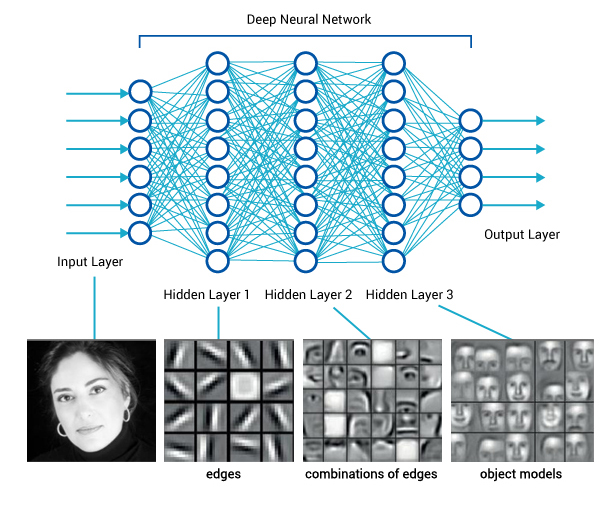
\includegraphics[width=0.5\textwidth]{neuraal-netwerk.png}
\end{figure}

\begin{itemize}
    \item The neurons are in one of three layers:
    \begin{itemize}
        \item Input layer
        \item Hidden layers
        \item Output layer
    \end{itemize}
    \item Every neuron is connected to every neuron of the next layer
    \item Every connection has a weight
    \item Deep Neural network $\Leftrightarrow$ multiple hidden layers
\end{itemize}

\subsection{History of deep learning}

\begin{figure}[H]
    \centering
    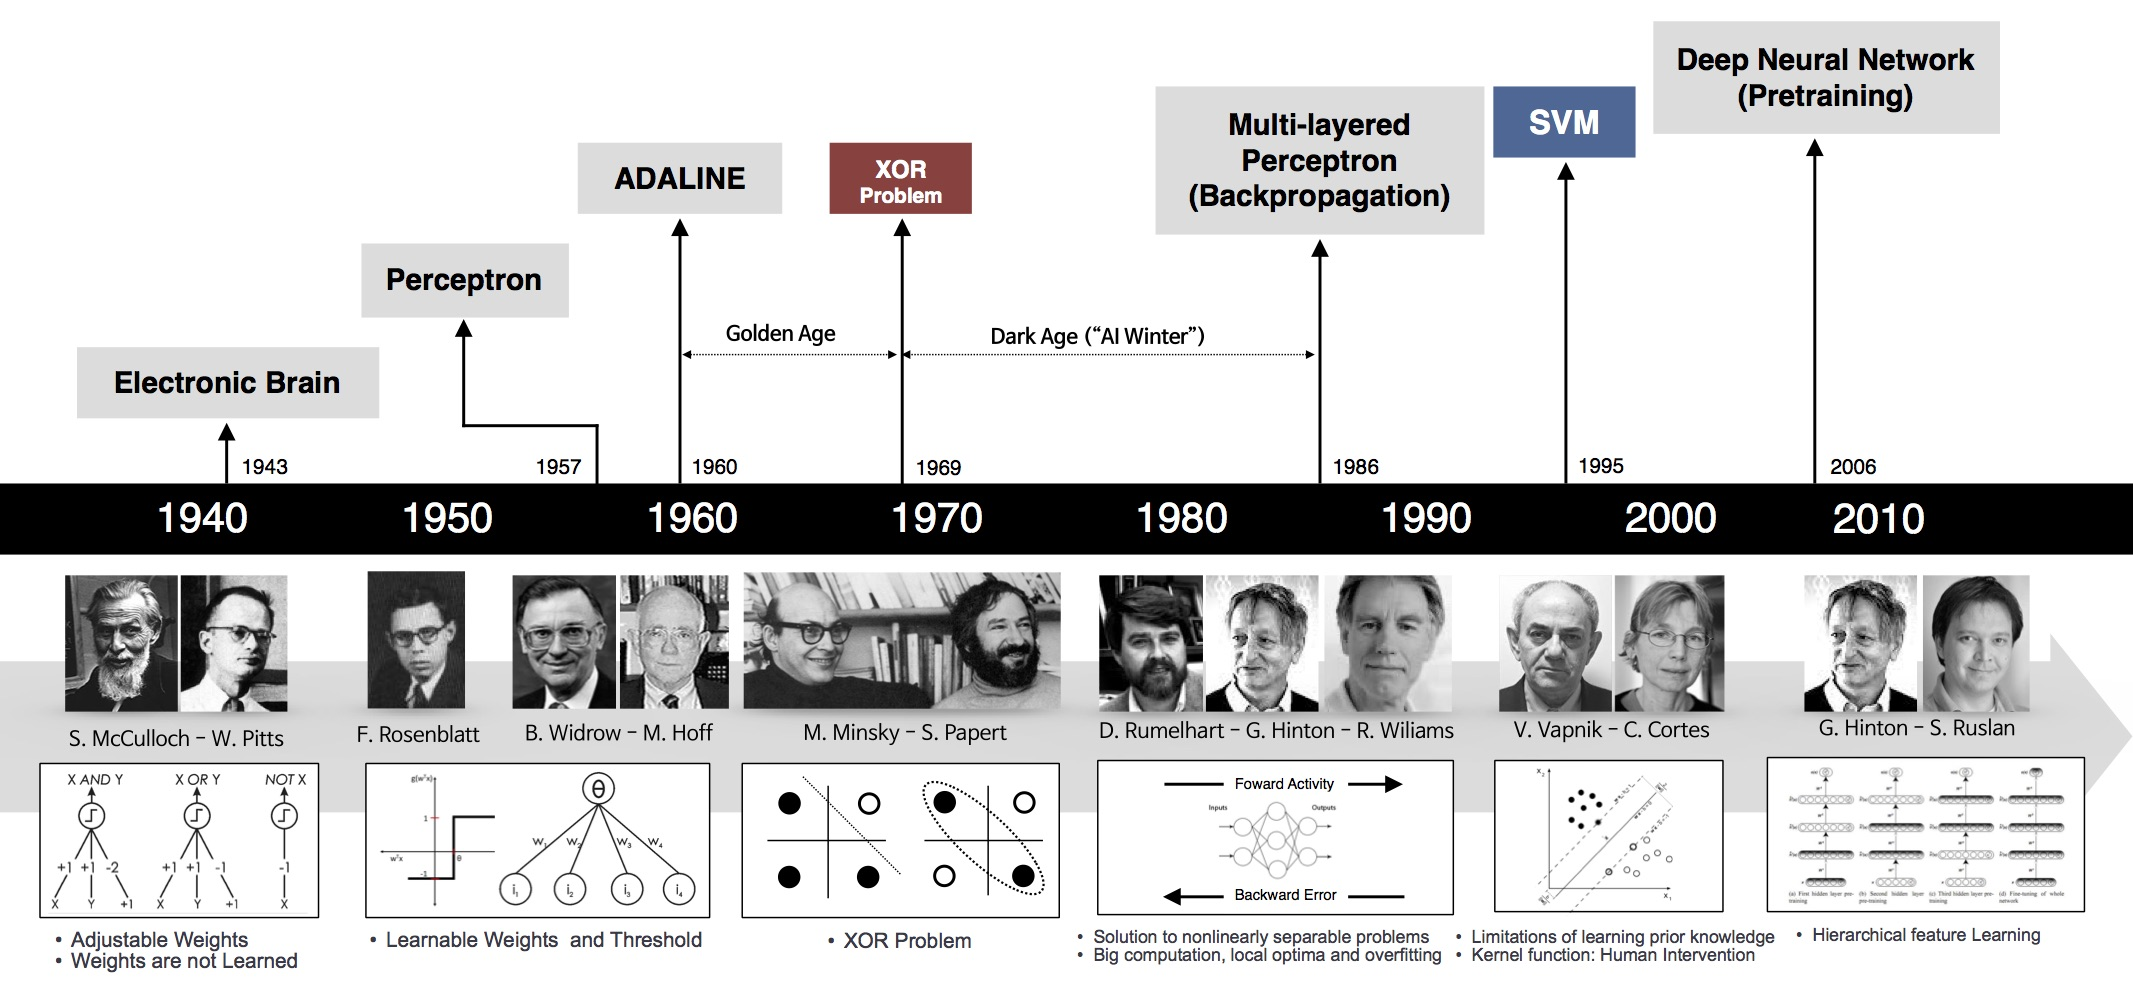
\includegraphics[width=0.5\textwidth]{deep-learning-history.png}
    \caption{\url{https://beamandrew.github.io/deeplearning/2017/02/23/deep_learning_101_part1.html}}
\end{figure}


\subsection{Deep learning architectures}

You can change many things about the components of a neural network. 
Here are some examples of popular architectures. The most important ones are in \textbf{bold}:

\begin{itemize}
    \item \textbf{Convolutional Neural Networks (CNN)}
    \item Capsule Network (CapsNet)
    \item Restricted Boltzmann Machine (RBM)
    \item \textbf{Autoencoder (AE)}
    \item Deep Belief Nets (DBN)
    \item \textbf{Recurrent Neural (Tensor) Network (RNTN)}
    \item \textbf{Long Short Term Memory (LSTM)}
    \item \textbf{Gated Recurrent Unit nets (GRU)}
    \item \textbf{Generatative Adversarial Nets (GAN)}
    \item \dots
\end{itemize}

\subsection{Biological model}

\begin{figure}[H]
    \centering
    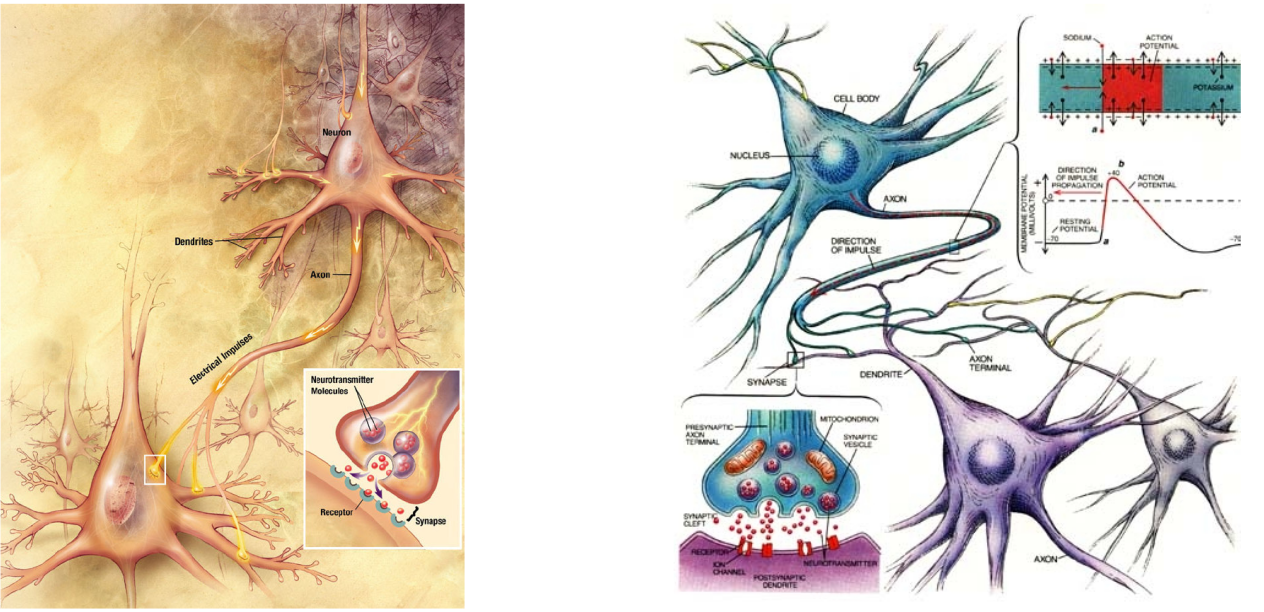
\includegraphics[width=0.5\textwidth]{biologisch-neuron.png}
    \caption{Anatomy of a biological neuron}
\end{figure}

\begin{itemize}
    \item Neural networks are inspired by our brains
    \item A neuron has multiple connections that can send signals to other neurons
    \item A neuron can send a weak or strong signal
\end{itemize}

\subsection{The artificial neuron}

\begin{figure}[H]
    \centering
    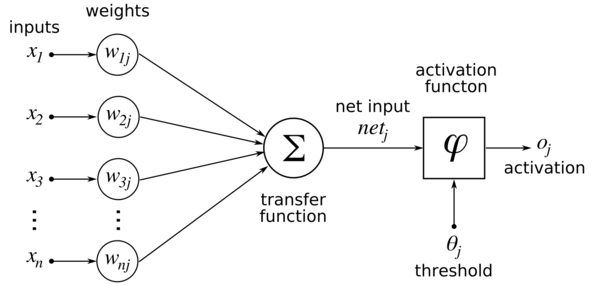
\includegraphics[width=0.5\textwidth]{neuron.png}
    \caption{Conceptual model}
\end{figure}

\begin{itemize}
    \item A neuron can receive multiple inputs
    \item Every input has a specified weight (= weak or strong signal)
    \item These inputs are multiplied by the weights, to then be used in a transfer function
    \item The transfer function is a mathematical formula that has a number as output
    \item That number is used as an input by an activation function. This functin will determine the final output
    \item \url{https://en.wikipedia.org/wiki/Activation_function}
\end{itemize}

\begin{figure}[H]
    \centering
    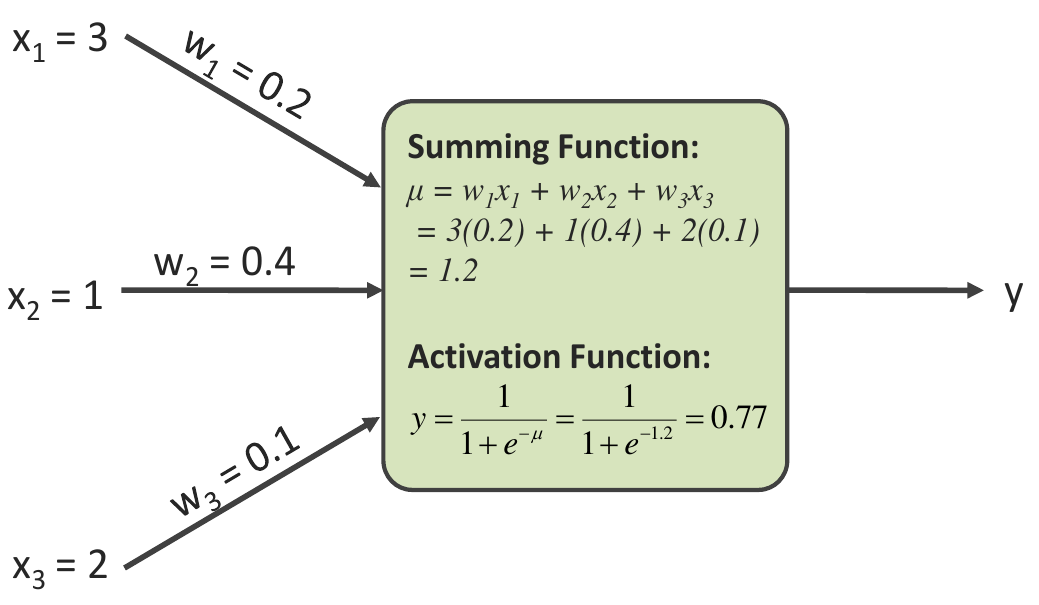
\includegraphics[width=0.5\textwidth]{neuron-voorbeeld.png}
    \caption{Example of a neuron, with a sigmoid function as activation function}
\end{figure}

\section{Logistic Regression}

\begin{theorem}
    Logistic regression is used to determine the probability of a certain sample 
    belonging to one of two classes.
    
    The name is a bit misleading: Logistic Regression is a classification technique, not regression. 
    The reason for this name is because regression is used to calculate the classification.
\end{theorem}

\subsection{The model}

Because the output is a probability, we're looking for a function $h_w$ so the model $h_w(x)$ :

\begin{center}
$0 \leq h_w(x) \leq 1$
\end{center}

\begin{itemize}
    \item $h_w(x)$ = estimated probability that $y=1$ for input $x$
    \item Example: $h_w(x) = 0.80$
    \begin{itemize}
        \item The model is 80\% sure that the sample belongs to class 1
        \item If you use a threshold of 50\%, the model will output 1
        \item If the prediction is less than that threshold of 50\%, the model will output 0
    \end{itemize}
\end{itemize}

\subsubsection{The logistic function}

\begin{equation}
h_w(x) = \frac{1}{1 + e^{-w^{\tau}x}}
\end{equation}

\begin{itemize}
    \item With $e =$ Euler's number = $\approx 2.718$
    \item This is a sigmoid function: the basic form for this is $\frac{1}{1+e^{-z}}$
    \item In our logistic function, $z$ equals $w^{\tau}x$
    \begin{itemize}
        \item This is equal to the solution of a linear regression function
        \item With $x =$ the sample values
        \item With $w =$ the weights that correspond to those values 
    \end{itemize}
\end{itemize}

\begin{figure}[H]
    \centering
    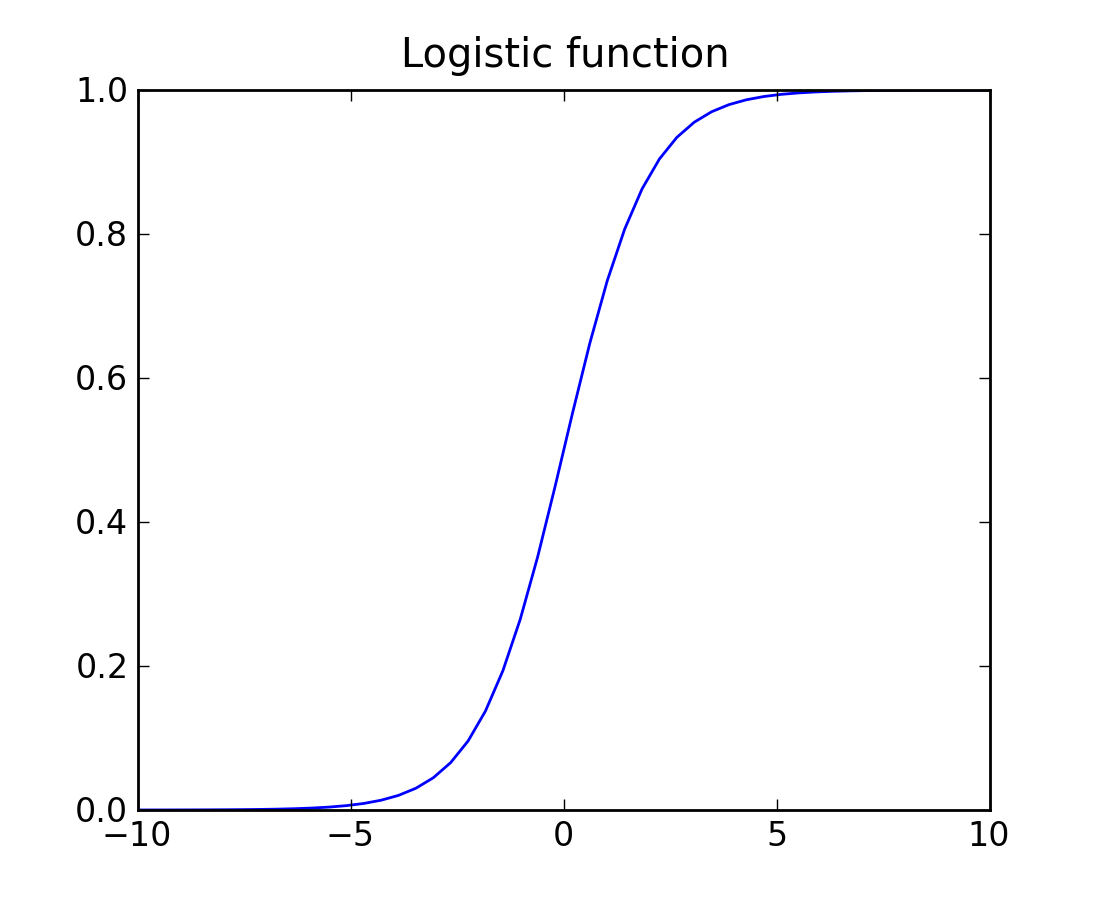
\includegraphics[width=0.3\textwidth]{logistic-regression.png}
    \caption{The logistic functie is evidently a sigmoid function or `S-function'}
\end{figure}

\begin{itemize}
    \item $y=1$ als $h_w(x) \geq 0.5 \Rightarrow w^{\tau}x \geq 0$
    \item $y=0$ als $h_w(x) < 0.5 \Rightarrow w^{\tau}x < 0$
\end{itemize}

\begin{figure}[H]
    \centering
    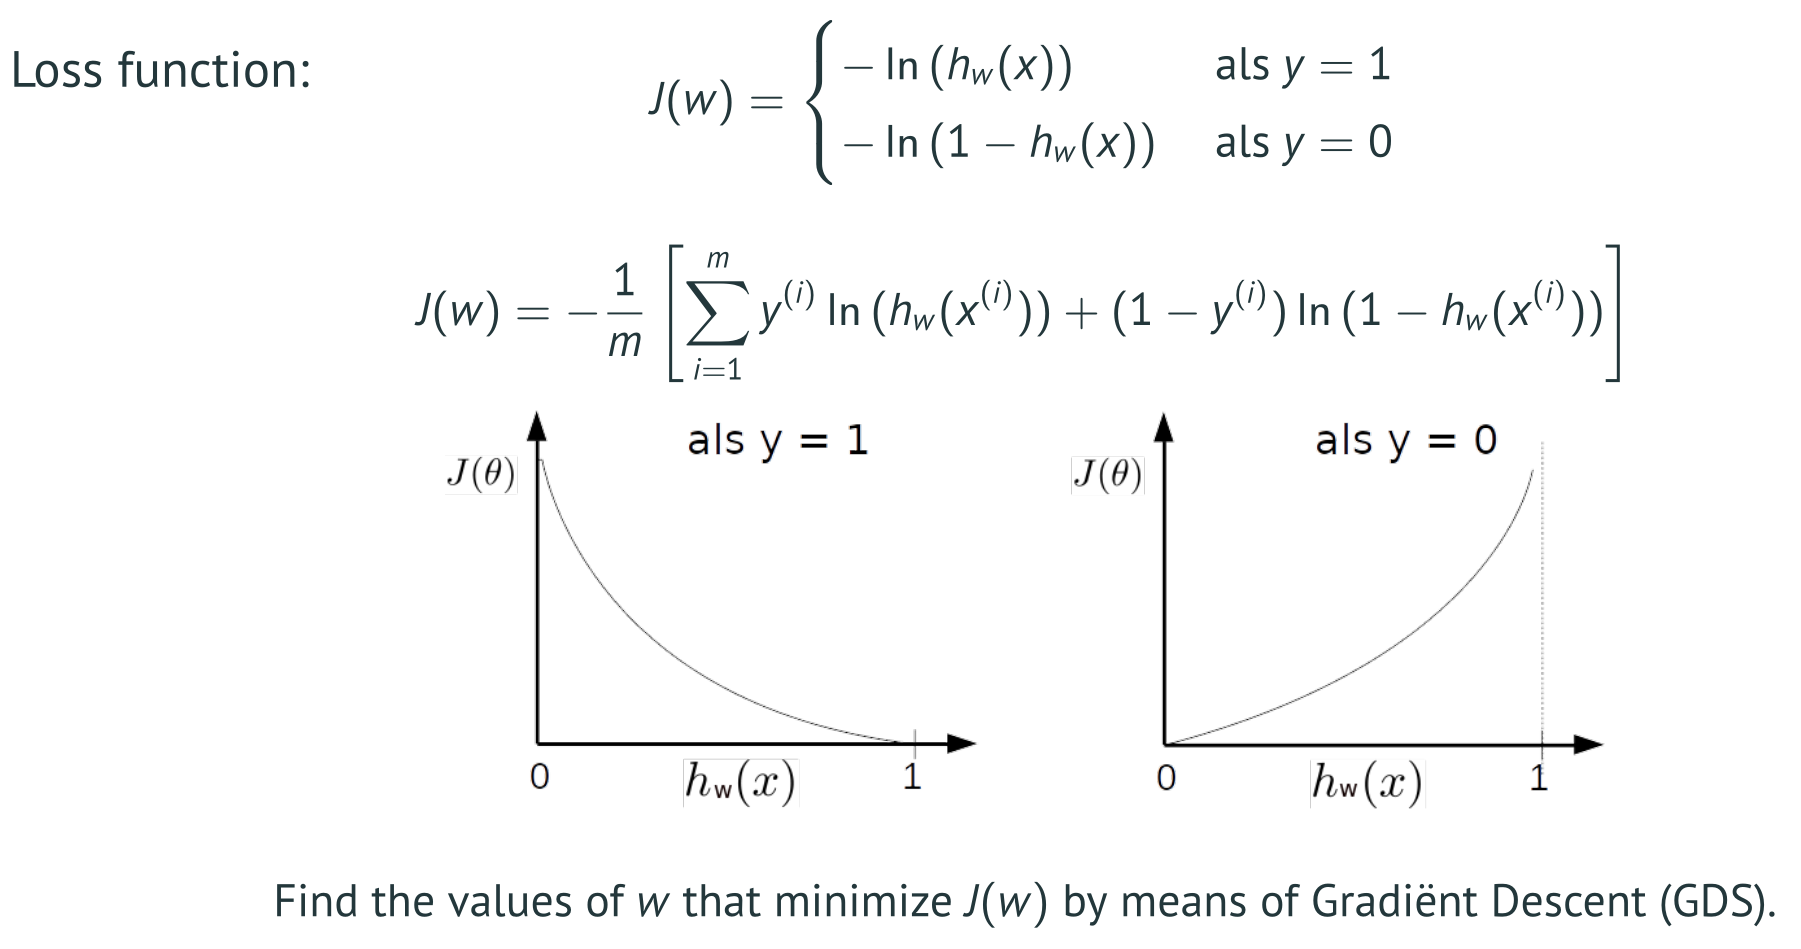
\includegraphics[width=0.5\textwidth]{img/logistic-regression-loss.png}
    \caption{Minizing the binary cross-Entropy loss function}
\end{figure}


\subsection{Logistic regression as a neuron}

\begin{figure}[H]
    \centering
    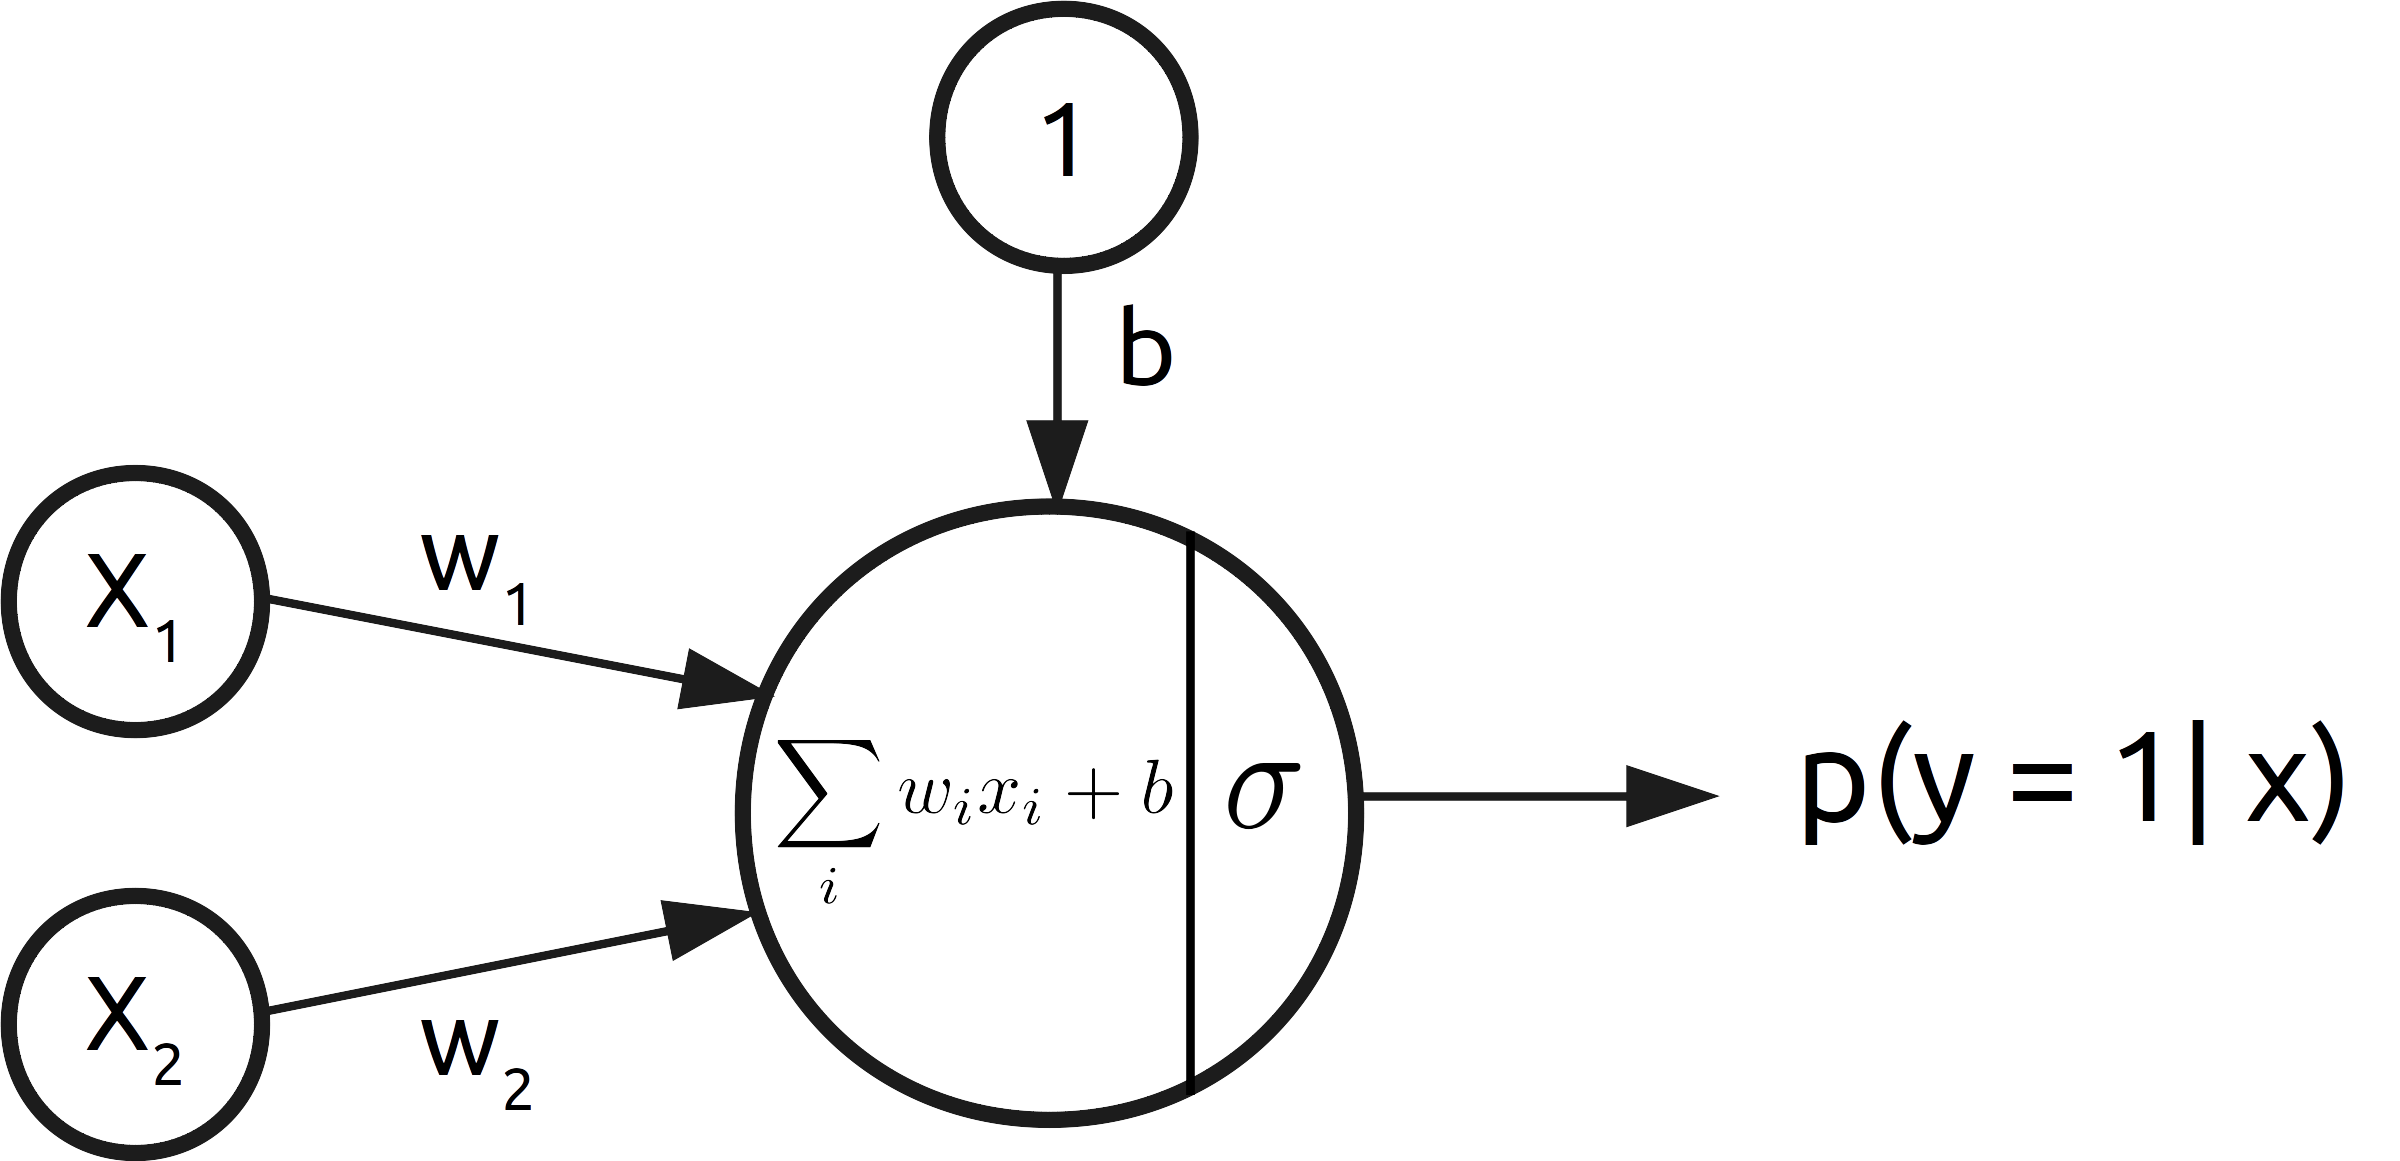
\includegraphics[width=0.5\textwidth]{logistic-regression-neuron.png}
    \caption{Logistic regression as a neuron}
\end{figure}



TODO: slides 19 - 25

\section{Properties of a neural network}

\subsection{Feedforward neural networks}

\subsubsection{Properties}

\begin{itemize}
    \item 1 or more (hidden) layers.
    \item Each neuron is in a layer is connected to every neuron in the next layer.
    \item Signals travel from input to output through the hidden layers. (feedforward)
    \item The neural network maps inputs to desired outputs.
\end{itemize}


\begin{figure}[H]
    \centering
    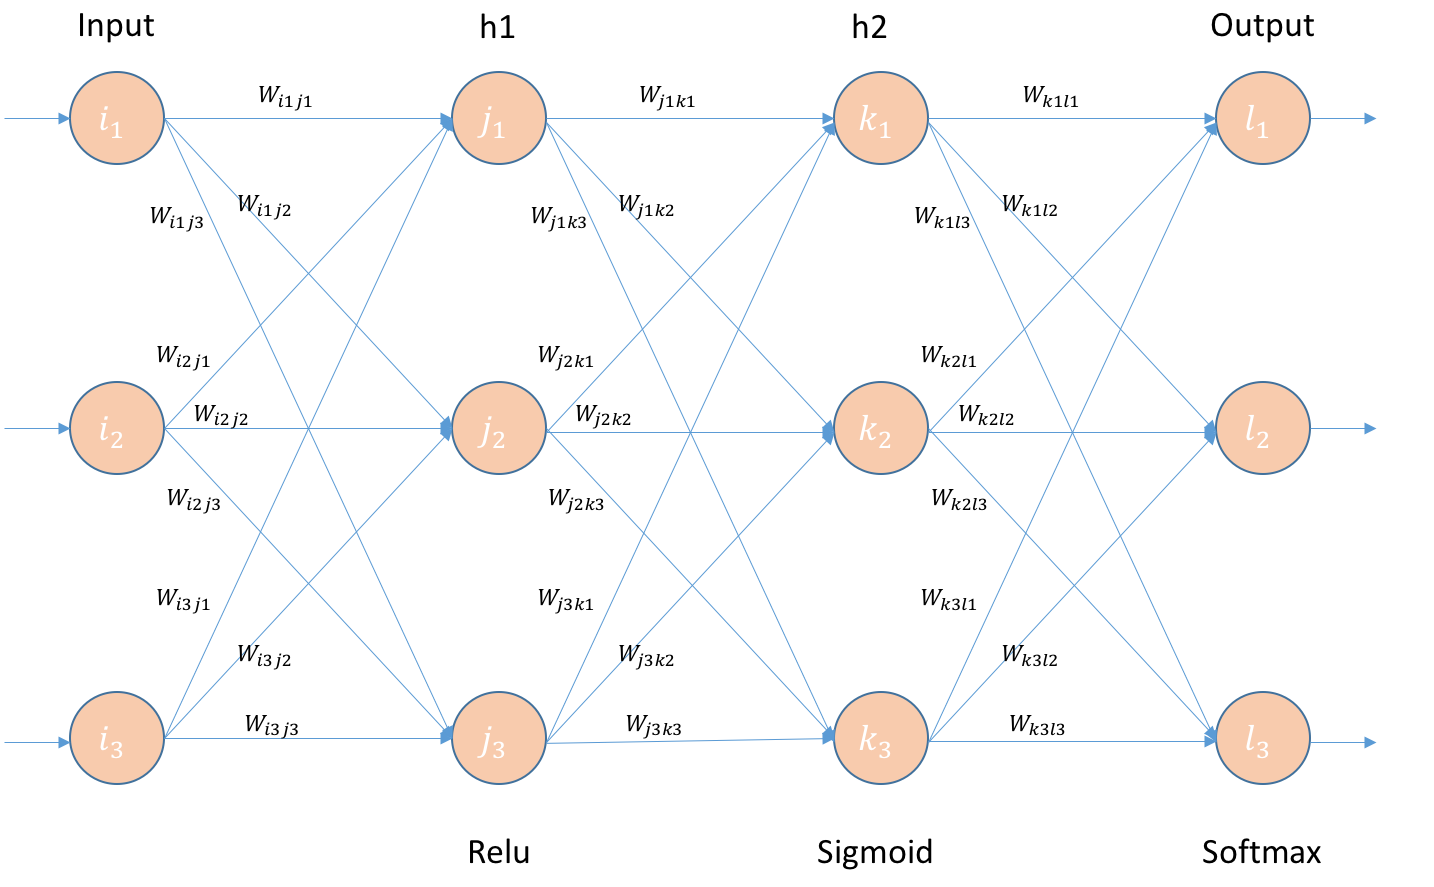
\includegraphics[width=0.5\textwidth]{feedforward-neural-network-properties.png}
    \caption{Feedforward neural network architecture}
\end{figure}

\subsubsection{MNIST example}

\begin{figure}[H]
    \centering
    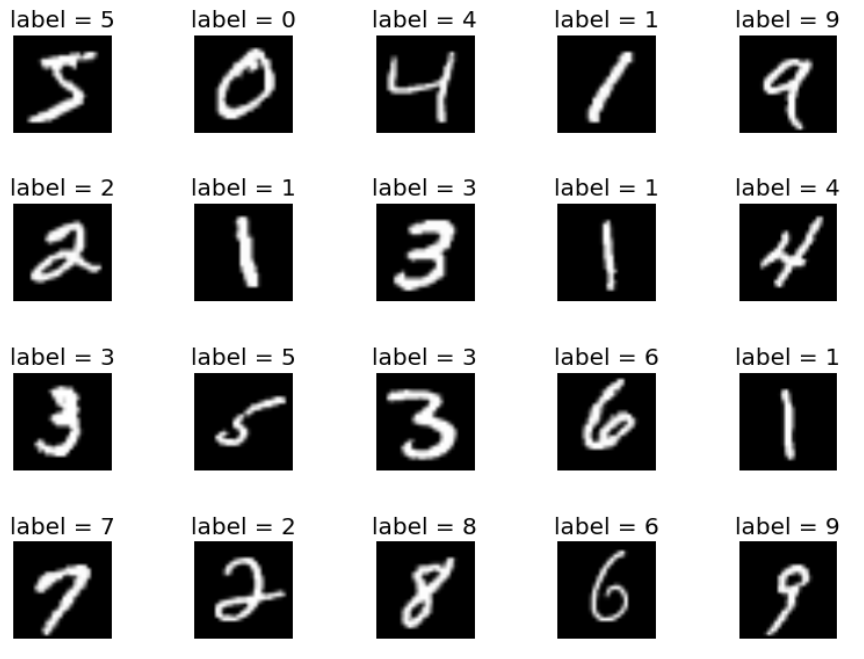
\includegraphics[width=0.4\textwidth]{mnist-neural.png}
    \caption{MNIST: dataset with labeled, handdrawn numbers}
\end{figure}

\begin{figure}[H]
    \centering
    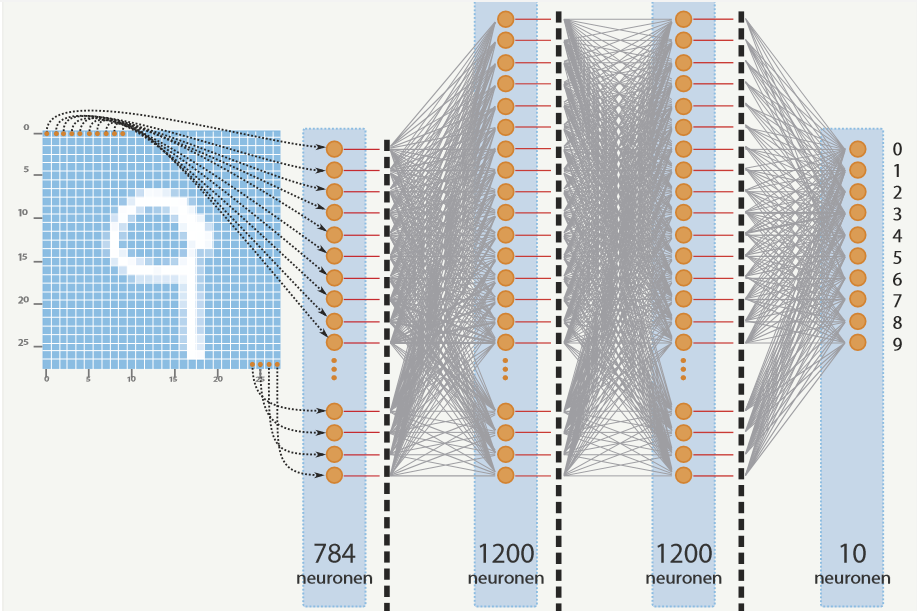
\includegraphics[width=0.5\textwidth]{mnist-neural2.png}
    \caption{Simplified example of a neural network}
\end{figure}

\begin{itemize}
    \item The numbers are drawn on a 28x28 grid (=784 input neurons)
    \item Every output (0-9) has a certain chance
    \item That chance determines how certain the model is that the given input is that number
    \item The chance is calculated using \textbf{backpropagation} (see later)
\end{itemize}

\subsubsection{One-hot encoding}

\begin{theorem}
    One-hot encoding is a technique to transform categorical features or targets to a more suitable format. 
    In a one-hot encoded target vector, the index of 1 represents the target label. All other values are 0.

    This is also used in neural networks.
\end{theorem}

\begin{figure}[H]
    \centering
    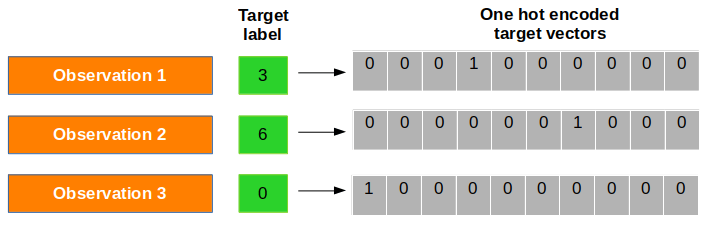
\includegraphics[width=0.4\textwidth]{one-hot.png}
\end{figure}

\begin{figure}[H]
    \centering
    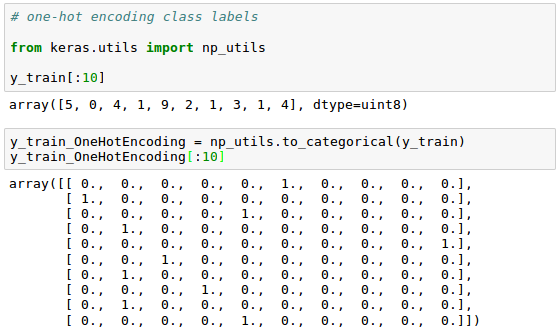
\includegraphics[width=0.5\textwidth]{one-hot2.png}
    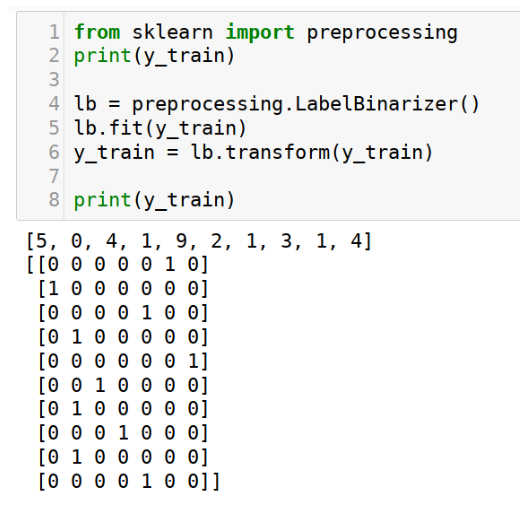
\includegraphics[width=0.3\textwidth]{neural-onehot.png}
    \caption{}
\end{figure}

\subsection{Multiclass classification}


How to classify with more than 2 classes?

\begin{figure}[H]
    \centering
    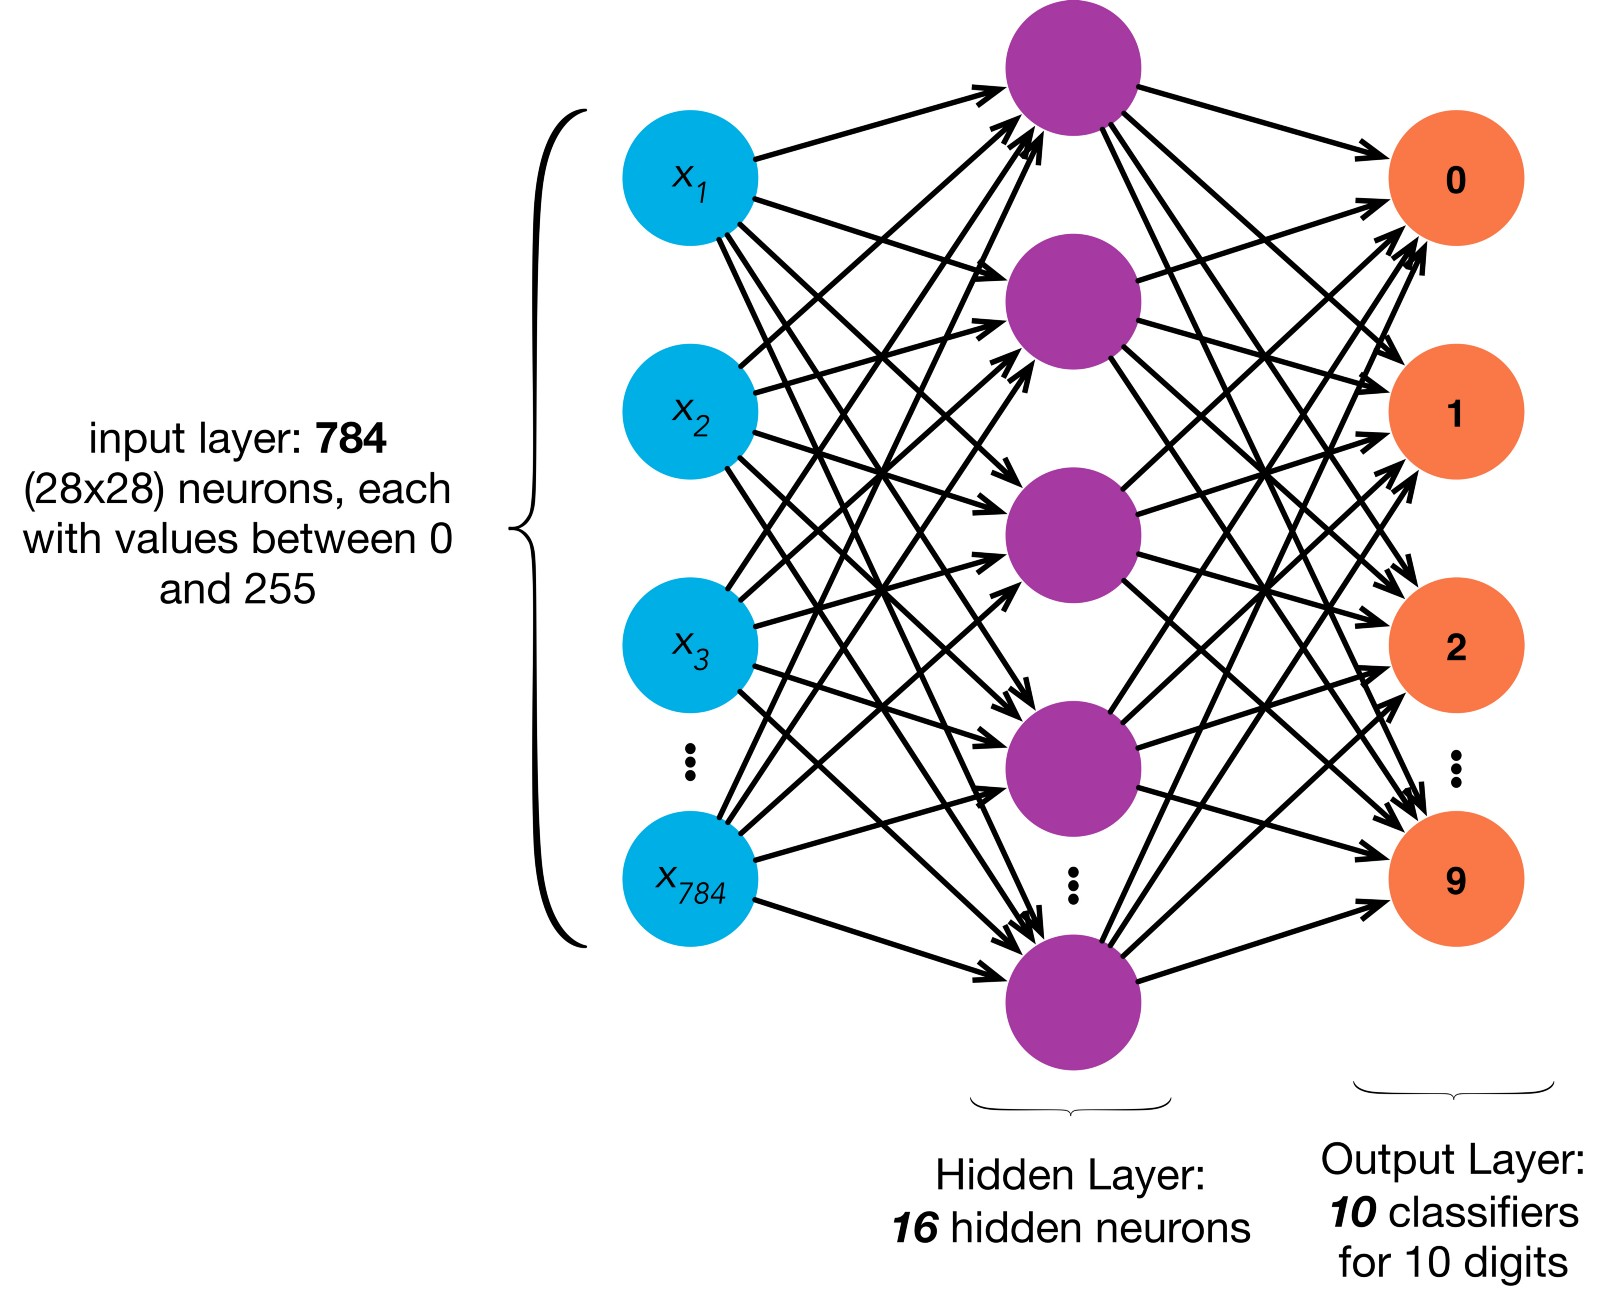
\includegraphics[width=0.5\textwidth]{multiclass-classification.png}
    \caption{}
\end{figure}

\begin{itemize}
    \item Sigmoid functions only allow for binary classification 
    \item We need a different function for multiclass classification with $K$ classes
    \item $\Rightarrow$ \textbf{Softmax function}
\end{itemize}

\begin{figure}[H]
    \centering
    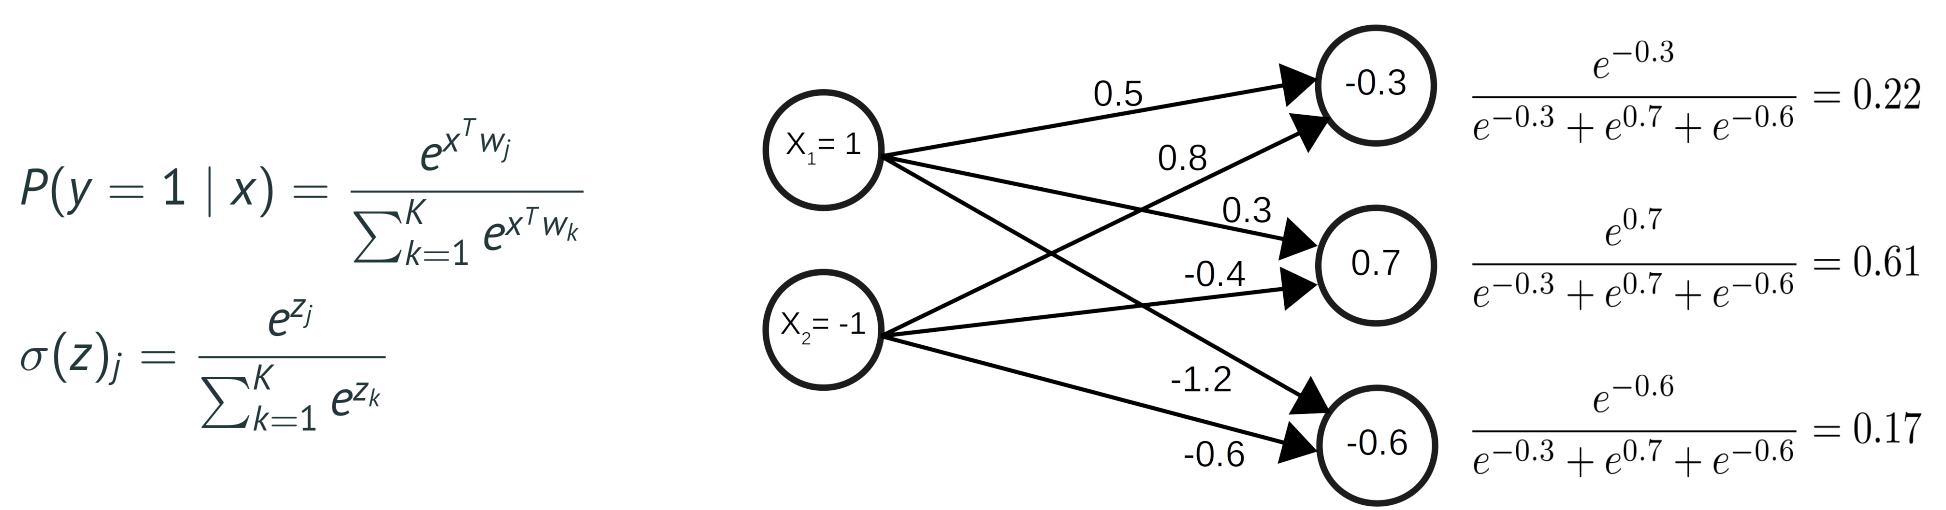
\includegraphics[width=0.85\textwidth]{img/softmax.png}
    \caption{Softmax function}
\end{figure}

TODO: more info about softmax

\begin{figure}[H]
    \centering
    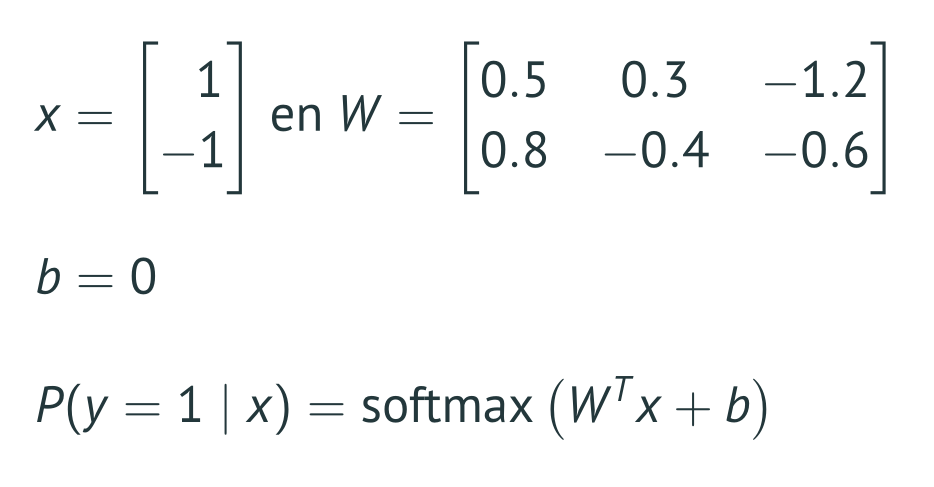
\includegraphics[width=0.5\textwidth]{img/softmax2.png}
    \caption{Output computation in vector notation}
\end{figure}


\subsubsection{Backpropagation}

\begin{theorem}
    Backpropagation is the most popular technique to train neural networks.
    It works by calculating an error (=loss) for every prediction, and to adjust the weights based on that error.
    
    The goal is to decrease the error as much as possible.
\end{theorem}

\begin{figure}[H]
    \centering
    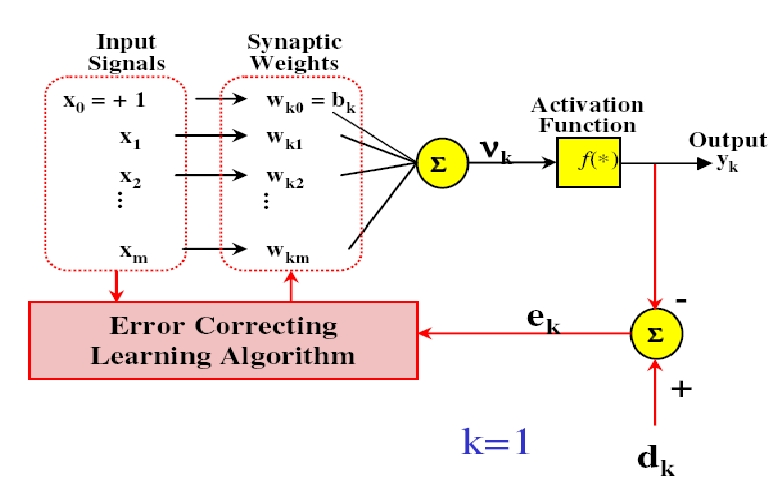
\includegraphics[width=0.5\textwidth]{img/backpropagation.png}
    \caption{}
\end{figure}

\begin{itemize}
    \item $\eta$ is the learning rate
    \item $0 < m \cdot \eta < 1$ with $m$ the number of inputs
    \item Error: $e_k(n) = d_k(n) - y_k(n)$
    \begin{itemize}
        \item Minimize the error $e_k(n)$
        \item $\epsilon(n) = \frac12 \sum_k e^2_k(n)$
        \item $\Delta W_{kj}(n) = \eta \cdot e_k(n) \cdot x_j(n)$
        \item Adjust the weight: $\Delta W_{kj}(n+1) = W_{kj}(n) + \Delta W_{kj}(n)$
    \end{itemize}
\end{itemize}

\url{https://becominghuman.ai/back-propagation-is-very-simple-who-made-it-complicated-97b794c97e5c}

\textbf{Using the MNIST example:}

\begin{itemize}
    \item In the output layer, the neural network assigns a probability to every number
    \item The prediction is made based on the highest chance.
    \item Suppose a certain number received too high a probability, and the true number too low a probability:
    \begin{itemize}
        \item The neural network will calculate the differences (=error)
        \item Next time, the neural network will try to keep the error as low as possible
        \item It does this by repeatedly adjusting the weights
        \item This process happens through all layers, from back to front $\Rightarrow$ \textbf{backpropagation}
    \end{itemize}
\end{itemize}

\begin{figure}[H]
    \centering
    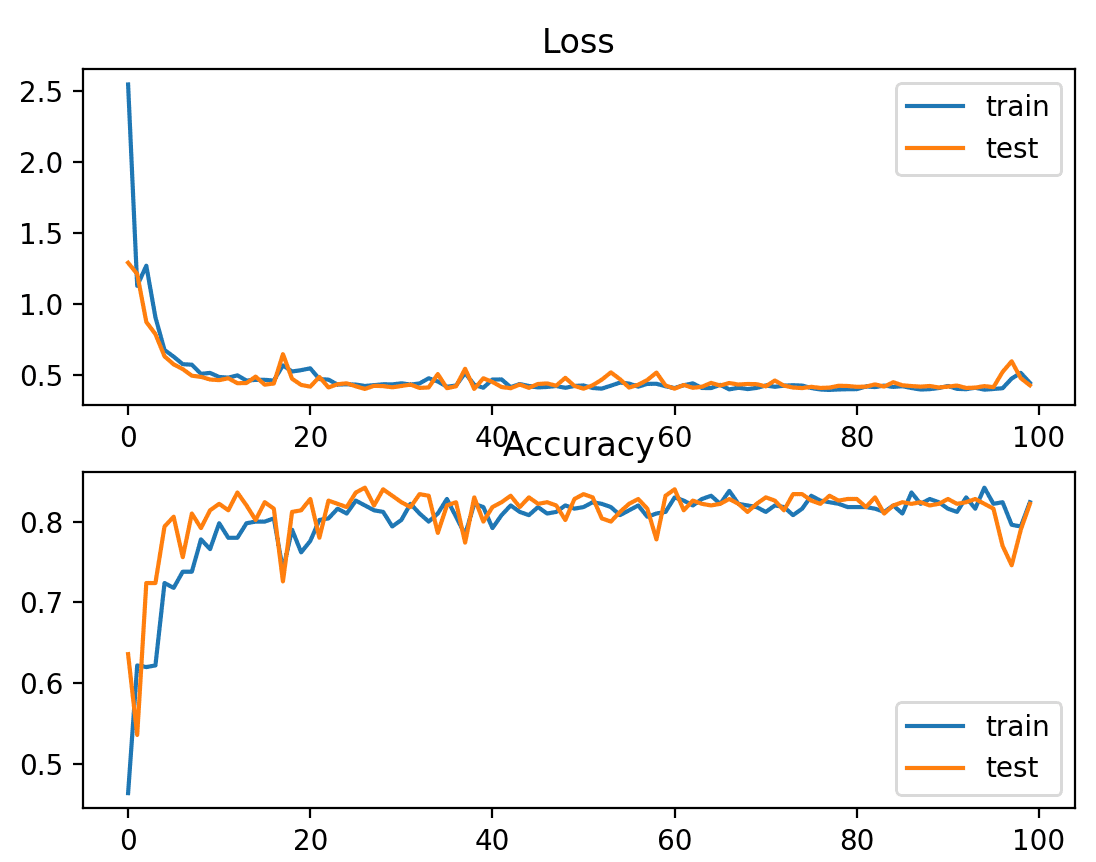
\includegraphics[width=0.5\textwidth]{backpropagation-error.png}
    \caption{The error function (=loss) in functie of the amount of training epochs}
\end{figure}


\begin{figure}[H]
    \centering
    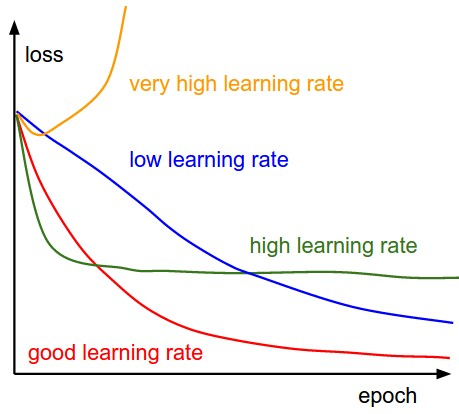
\includegraphics[width=0.4\textwidth]{backpropagation-learning-rate.png}
    \caption{Impact of the learning rate to the loss. During training, the learning rate keeps changing.}
\end{figure}

\subsection{Activation function}

\begin{figure}[H]
    \centering
    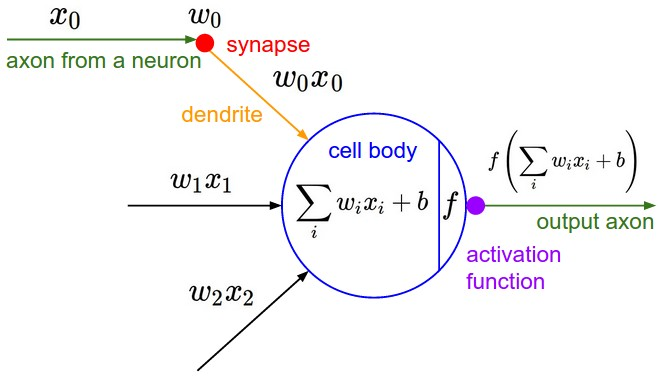
\includegraphics[width=0.5\textwidth]{activation-function.png}
\end{figure}


\begin{theorem}
    The activation function of a neuron defines the output of that neuron using a mathematical function.
    The inputs are multiplied by their weight, and are then summed up by the transfer function.
    The output of that transfer function is used as an input by the activation function.
\end{theorem}

There are various functions that each have a specific output range (possible y-values):


\begin{itemize}
    \item Step function: 0 or 1
    \item Linear function: $-\infty$ to $+\infty$
    \item Sigmoid function: $0$ to $1$
    \item Hyperbolic tangent (tanh): $-1$ to $1$
    \item ReLu: $0$ to $+\infty$
    \item Leaky ReLu: $-\infty$ to $+\infty$
\end{itemize}



\end{document}